\documentclass{subfile}
\begin{document}
\subsection{Binary Tree Sort}\label{C:BT}
\begin{align*}
  \text{Best-Case Performance}\quad &O\left(n\log n\right)\\
  \text{Average Performance}\quad &O\left(n\log n\right)\\
  \text{Worst-Case Performance}\quad &O\left(n^{2}\right)\\
  \text{Worst-Case Space Complexity}\quad &O\left(n\right)
\end{align*}
\begin{multicols}{2}
  Binary tree sort is an algorithm that utilizes the binary tree structure in order to sort the items into the correct order. Figure \ref{C:BT:1} is an example of a binary tree structure, where each node has up to two child nodes. Using this structure a binary tree can be created to sort an unsorted array of elements. Through the process of creating a binary tree the elements are sorted as they are inserted into the tree. A simple recursive algorithm can be used to insert elements into the binary tree. Once all elements have been inserted into the binary tree to retrieve the sorted array, the elements of the binary array must be read from left to right.
  \begin{Figure}
    \centering
    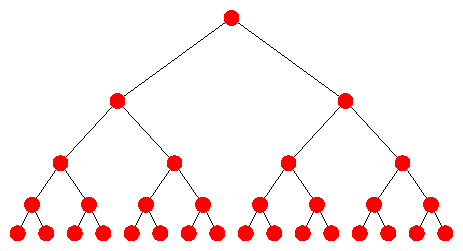
\includegraphics[width=\linewidth]{comparison_sorts/binary_tree/img1.pdf}
    \captionof{figure}{Example of Binary Tree structure}
  \end{Figure}\label{C:BT:1}
  \par
  The process of adding one item to a binary search tree is on average $O\left(\log n\right)$ so adding $n$ items to the tree will average to $O\left( n \log n \right)$. However, adding an item to an unbalanced tree needs $O\left( n\right)$ time, meaning that a worst case for adding $n$ items to a tree will be $O\left( n^{2} \right)$. This worst case performance occurs when the algorithm is acting on an already sorted array.
  \par
  Pseudocode for the Binary Tree algorithm is shown below in Algorithm \ref{C:BT:2}. The core of the algorithm is a object ($root$) that contains a left and right sub-copy of itself ($leftTree$, $rightTree$). The function $BinaryTree$ takes in an array of items to be sorted, it them adds each one to the binary tree ($root$), and then when the tree is completed it can be read, which in turn returns the sorted array. The function $Insert$ takes a binary tree ($tree$) to add a item ($value$) to. First this function checks to see if the binary tree is empty, and if so, it creates the root with the item to be inserted. If the binary tree is not empty, then the function determines if the item belongs in the left sub-tree, or the right sub-tree. If the item is less than the item in the root position of the binary tree, then $Insert$ function is run with the left sub-tree as the new root, and otherwise the function is run with the right sub-tree as the new root. The $ReadTree$ function traverses the binary tree from left most to right most node, by recursively entering the left branch if it exists, then adding the current node to the array, then recursively entering the right branch if it exists.
  \par
  Source code examples of Binary Tree sort can be found in \ref{APENDIX:BT}.
\end{multicols}
\newpage
\begin{algorithm}
  \caption{Binary Tree Pseudocode}\label{C:BT:2}
  \begin{algorithmic}[1]
  \Function{BinaryTree}{$a$}
    \State $root\gets null$
    \For{$i=0$ to $n$}
      \State \Call{Insert}{$root$,$a[i]$}
    \EndFor
    \State $a \gets $\Call{ReadTree}{$root$, $a$}
  \EndFunction
  \Function{Insert}{$tree$, $value$}
    \If{$tree=null$}
      \State $tree.value \gets value$
      \State $tree.leftTree \gets null$
      \State $tree.rightTree \gets null$
    \ElsIf{$tree.value\leq value$}
      \State \Call{Insert}{$tree.leftTree$, $value$}
    \Else
      \State \Call{Insert}{$tree.rightTree$, $value$}
    \EndIf
    \State \Return $tree$
  \EndFunction
  \Function{ReadTree}{$tree$, $a$}
    \If{$tree\neq null$}
      \State \Call{ReadTree}{$tree.leftTree$, $a$}
      \State $a$ append $tree.value$
      \State \Call{ReadTree}{$tree.rightTree$, $a$}
    \EndIf
    \State \Return $a$
  \EndFunction
\end{algorithmic}
\end{algorithm}
\newpage
\begin{multicols}{2}
  \begin{tikzpicture}
    \begin{axis}[scaled ticks=false,
        width=\linewidth,
        samples=100,
        xmin=1,
        xmax=100,
        ymin=0,
        ymax=1000,
        domain=1:100,
        restrict y to domain=0:1000,
        xlabel={$Elements$},
        ylabel={$Operations$},
        xticklabels={,,},
        yticklabels={,,},
      ]
      \addplot[color=red]{x^2};
      \addlegendentry{$n^2$}
      \addplot[color=yellow]{x * log10(x)};
      \addlegendentry{$n\log(n)$}
      \addplot[color=green]{x * log10(x)};
      \addlegendentry{$n\log(n)$}
      \addplot[color=blue]{x};
      \addlegendentry{$n$}
    \end{axis}
  \end{tikzpicture}
  \par
  This is a plot of the theoretical run times for Binary tree sort for increasing numbers of elements in the array. The worst case run times grow extreamly rapidly compaired to the averge and best case run times (which are the same). The rate of growth for the worst case run time is very poor, and the average and best case run times are still not optimal, and grow quickly. The plot for the space complexity also grows quite rapidly.
\end{multicols}
\begin{multicols}{2}
  \begin{tikzpicture} 
    \begin{axis}[scaled ticks=false,
        width=\linewidth,
        xlabel={$Elements$},
        ylabel={$Operations$},
      ]
      \addplot+[color=red, mark=none] table[x=n,y=time] {comparison_sorts/binary_tree/data.dat};
      \addplot+[color=green, mark=none] table[x=n,y=comparisons] {comparison_sorts/binary_tree/data.dat};
      \addplot+[color=blue, mark=none] table[x=n,y=vec_access] {comparison_sorts/binary_tree/data.dat};
    \end{axis}
  \end{tikzpicture}
\end{multicols}
\newpage
\end{document}
